\documentclass[dvipdfmx]{jreport}
\usepackage{tikz}
\usetikzlibrary{intersections,calc,arrows.meta}
\usepackage{graphicx}
\usepackage{xcolor}
\usepackage{amsmath}
\usepackage{amsfonts}
\usepackage{amssymb}
\usepackage{amsthm}
\usepackage{bm}
\usepackage{romannum}
\usepackage[dvipdfmx,hidelinks]{hyperref}
\usepackage{pxjahyper}
\usepackage{framed}
\usepackage{pifont}
\usepackage{float}
\newenvironment{claim}[1]{\par\noindent\underline{Claim:}\space#1}{}
\newenvironment{claimproof}[1]{\par\noindent\underline{Proof:}\space#1}{\hfill $\square$}
\DeclareMathOperator{\spn}{\mathbb{Q}-span}
\begin{document}
\pagenumbering{arabic}
\title{年末年始に何もやりたくないのにこの課題をやらせるのは人権侵害にあたる}
\author{習近平}
\date{2021年12月25日}
\maketitle
\newpage
\tableofcontents
\addcontentsline{toc}{chapter}{目次}
\setcounter{chapter}{3}
\newpage
\section{問題1 畳み込みの結合律を示せ}
$f,g,h : \mathbb{R} \to \mathbb{R} $を連続函数とする。写像$\phi_A : \mathbb{R}^2 \to \mathbb{R}^2$の表現行列$A$を次のように定める:
$$
A = 
\left( 
\begin{array}{cc}
0 & 1\\
1 &1 \\
\end{array}
\right)
$$
また $x \in \mathbb{R} $に対し、$\mathbb{R}^2$ の部分集合 $D= \left\{ (s,t) \in \mathbb{R}^2 \mid 0 \le s \le x-t, 0 \le t \le x \right\}$,
$E= \left\{(m,n) \in \mathbb{R}^2 \mid \textcolor{red}{0 \le m \le n \le x} , 0 \le n \le x \right\}$とする。\\
このもとで問題を示す:
\begin{proof}
\begin{equation}
\begin{aligned}
\int_0^x \left( f*g \right) (x-t) h(t)dt &= \int_0^x \left( \int_0^{x-t} f(x-t-s) g(s) ds \right) h(t) dt \\
					 &= \iint_{D} f(x-t-s)g(s)h(t)dsdt
\end{aligned}\label{eq:1}
\end{equation}
	\begin{figure}[H]
		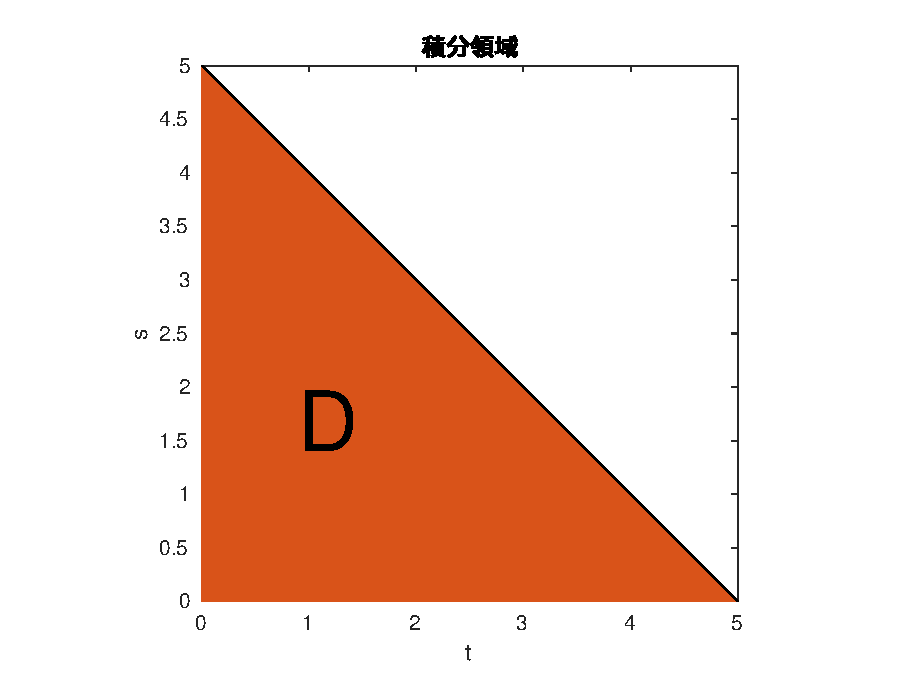
\includegraphics[scale=0.3]{1.eps}
		
\includegraphics[scale=0.3]{2.eps}
		\caption{写像のイメージ図 \newline
		{\footnotesize  あくまでイメージなので、座標に数値がついても文句を言わないで、ちゃんとした証明は集合$D,E$を用いて定式化したため、無断減点行為を固く禁じる} }
	\end{figure}
	また、$\phi_A(D)=E$が成り立ち、$\det(A)=-1$より、$\phi_A$が全単射であることがわかる。したがって式\ref{eq:1}の続きは以下のようになる:
	\begin{equation}
		\begin{aligned}
			\int_0^x \left( f*g \right) (x-t) h(t)dt &=  \iint_{D} f(x-t-s)g(s)h(t)dsdt\\
								 &=  \iint_{E} f(x-n)g(n-m)h(m)|A^{-1}|dmdn \\
								 &=  \int_0^x f(x-n) \left( \int_0^n g(n-m)h(m) dm \right) dn\\
								 &=  \int_0^xf(x-n) (g*h)(n)dn\\
								 &=  \left(f*(g*h) \right)(x)
		\end{aligned}
	\end{equation}
以上より、問題の主張を示せた。
\end{proof}
\newpage
\section{つまらない計算問題その一}
$0<a<b,D= \{ (x,y) \in \mathbb{R}^2 \mid a\le x+y \le b, x\ge 0, y\ge 0 \}$とする。次の重積分を求めよ:
$$
\iint_D \frac{x^2 +y^2}{(x+y)^3}dxdy
$$
やはり線形写像を用いて、変数変換を行いたい。この時、写像$\phi_A : \mathbb{R}^2 \to \mathbb{R}^2$の表現行列$A$を次のように定める:
$$
A=
\left(
\begin{array}{cc}
	1 & 1\\
	1 & -1\\
\end{array}
\right)
$$
集合$E=\{ (s,t) \in \mathbb{R}^2 \mid a \le s \le b, -s \le t \le s\}$とする。この時、$\det(A) = 2$より、$\phi_A $は全単射であり、また$\phi_A(D) =E$より:
$$
\begin{aligned}
	\iint_D \frac{x^2 +y^2}{(x+y)^3}dxdy &= \frac{1}{2} \iint_E \frac{s^2 +t^2}{s^3}|A^{-1}|dtds\\
					     &=\frac{1}{4} \int_a^b \left( \int_{-s}^{s} \frac{1}{s} +\frac{t^2}{s^3} dt \right) ds\\
					     &=\frac{1}{2} \int_a^b \left[ \frac{t}{s} + \frac{t^3}{3s^3} \right]_{t=0}^sds \\
					     &=\frac{1}{2} \int_a^b \frac{4}{3} ds =\frac{2(b-a)}{3}
\end{aligned}
$$
\newpage
\section{つまらない計算問題その二}
次のように定義される曲線で囲まれる$\mathbb{R}^2$内の領域の面積を求めよ:
$$
(x^2 +y^2)^2 = x^2 -y^2
$$
この領域は集合$D = \{ (x,y) \in \mathbb{R}^2 \mid (x^2 +y^2)^2 \le x^2 -y^2\}$で表せる。次に$D$の点を$ 0 \le \theta < 2\pi,r\in \mathbb{R}_{\ge 0} $の範囲で、極座標変換を考えると
\begin{equation}
	\begin{cases}
		x=r\cos\theta\\
		y=r\sin \theta
	\end{cases}
\end{equation}
集合$E =\{(r,\theta ) \in \mathbb{R}^2 \mid 0< r^2 \le  \cos 2\theta , \theta \in (0,\frac{\pi}{4} ] \cup [\frac{3\pi}{4},\frac{5\pi}{4}]\cup[\frac{7\pi}{4},2\pi) \}\cup\{0\}$は先程の極座標変換で、集合$D$の像$F$は$E$の部分集合であるしかも$E\setminus F$の体積は0となる。この時積分を実行すると次のようになる:
\begin{equation}
	\begin{aligned}
		\iint_D dxdy &= \iint_E rdrd\theta\\
			     &= \frac{1}{2} \left( \int_0^{\frac{\pi }{4}} \cos2\theta d\theta  
			      +\int_{\frac{3\pi}{4}}^{\frac{5\pi }{4}} \cos2\theta d\theta  
			      +\int_{\frac{7\pi }{4}}^{ 2 \pi } \cos2\theta d\theta  \right)\\
			     &=\frac{1}{4}+\frac{1}{2}+\frac{1}{4}=1
	\end{aligned}
\end{equation}
以上より、曲線に囲まれる部分の面積は$1$である。
\newpage
\section{\#雑談}
年末年始はゆっくり休みたいのに、この課題を出すことは人権侵害にあたるだろう。線形代数学B、物理学B、解析学B、解析学序論A、情報理学入門、いずれも課題が多量に出ており、休みとなるべき時間に作業しなければいけない苦痛しかない状態になっています。ちなみにこのレポートはカップルでデートするはずのクリスマスに完成されたものです。(カップルは存在しないのは原因ですが) \LaTeX で作成したこのレポートに添字ミスとかがあるかもしれないがご了承ください。第一問で変数変換したあともリーマン可積分であることを示さなければいけないだけど,講義でもごまかしたから証明はこのぐらいにしておきます.最後の一問で全単射であることを確認する作業はあまりにも時間かかると思うため、省略させていただきました。長い時間取らせていただきまして、お疲れ様でした。ではこのレポートを検閲している皆様に良い2022を過ごせることを心よりお祈り申し上げます。

\end{document}
                              
 
